%----------------------------------------------------------------------------------------
%	PACKAGES AND OTHER DOCUMENT CONFIGURATIONS
%----------------------------------------------------------------------------------------

\documentclass{article}
\usepackage{graphicx}
%%%%%%%%%%%%%%%%%%%%%%%%%%%%%%%%%%%%%%%%%
% Lachaise Assignment
% Structure Specification File
% Version 1.0 (26/6/2018)
%
% This template originates from:
% http://www.LaTeXTemplates.com
%
% Authors:
% Marion Lachaise & François Févotte
% Vel (vel@LaTeXTemplates.com)
%
% License:
% CC BY-NC-SA 3.0 (http://creativecommons.org/licenses/by-nc-sa/3.0/)
% 
%%%%%%%%%%%%%%%%%%%%%%%%%%%%%%%%%%%%%%%%%

%----------------------------------------------------------------------------------------
%	PACKAGES AND OTHER DOCUMENT CONFIGURATIONS
%----------------------------------------------------------------------------------------

\usepackage{amsmath,amsfonts,stmaryrd,amssymb} % Math packages

\usepackage{enumerate} % Custom item numbers for enumerations

\usepackage[ruled]{algorithm2e} % Algorithms

\usepackage[framemethod=tikz]{mdframed} % Allows defining custom boxed/framed environments

\usepackage{listings} % File listings, with syntax highlighting
\lstset{
	basicstyle=\ttfamily, % Typeset listings in monospace font
}

%----------------------------------------------------------------------------------------
%	DOCUMENT MARGINS
%----------------------------------------------------------------------------------------

\usepackage{geometry} % Required for adjusting page dimensions and margins

\geometry{
	paper=a4paper, % Paper size, change to letterpaper for US letter size
	top=2.5cm, % Top margin
	bottom=3cm, % Bottom margin
	left=2.5cm, % Left margin
	right=2.5cm, % Right margin
	headheight=14pt, % Header height
	footskip=1.5cm, % Space from the bottom margin to the baseline of the footer
	headsep=1.2cm, % Space from the top margin to the baseline of the header
	%showframe, % Uncomment to show how the type block is set on the page
}

%----------------------------------------------------------------------------------------
%	FONTS
%----------------------------------------------------------------------------------------

\usepackage[utf8]{inputenc} % Required for inputting international characters
\usepackage[T1]{fontenc} % Output font encoding for international characters

\usepackage{XCharter} % Use the XCharter fonts

%----------------------------------------------------------------------------------------
%	COMMAND LINE ENVIRONMENT
%----------------------------------------------------------------------------------------

% Usage:
% \begin{commandline}
%	\begin{verbatim}
%		$ ls
%		
%		Applications	Desktop	...
%	\end{verbatim}
% \end{commandline}

\mdfdefinestyle{commandline}{
	leftmargin=10pt,
	rightmargin=10pt,
	innerleftmargin=15pt,
	middlelinecolor=black!50!white,
	middlelinewidth=2pt,
	frametitlerule=false,
	backgroundcolor=black!5!white,
	frametitle={scene-start.cpp},
	frametitlefont={\normalfont\sffamily\color{white}\hspace{-1em}},
	frametitlebackgroundcolor=black!50!white,
	nobreak,
}

% Define a custom environment for command-line snapshots
\newenvironment{commandline}{
	\medskip
	\begin{mdframed}[style=commandline]
}{
	\end{mdframed}
	\medskip
}

%----------------------------------------------------------------------------------------
%	COMMAND LINE ENVIRONMENT
%----------------------------------------------------------------------------------------

% Usage:
% \begin{commandlineF}
%	\begin{verbatim}
%		$ ls
%		
%		Applications	Desktop	...
%	\end{verbatim}
% \end{commandlineF}

\mdfdefinestyle{commandlineF}{
	leftmargin=10pt,
	rightmargin=10pt,
	innerleftmargin=15pt,
	middlelinecolor=black!50!white,
	middlelinewidth=2pt,
	frametitlerule=false,
	backgroundcolor=black!5!white,
	frametitle={fStart.glsl},
	frametitlefont={\normalfont\sffamily\color{white}\hspace{-1em}},
	frametitlebackgroundcolor=black!50!white,
	nobreak,
}

% Define a custom environment for command-line snapshots
\newenvironment{commandlineF}{
	\medskip
	\begin{mdframed}[style=commandlineF]
	}{
	\end{mdframed}
	\medskip
}

%----------------------------------------------------------------------------------------
%	COMMAND LINE ENVIRONMENT
%----------------------------------------------------------------------------------------

% Usage:
% \begin{commandlineV}
%	\begin{verbatim}
%		$ ls
%		
%		Applications	Desktop	...
%	\end{verbatim}
% \end{commandlineV}

\mdfdefinestyle{commandlineV}{
	leftmargin=10pt,
	rightmargin=10pt,
	innerleftmargin=15pt,
	middlelinecolor=black!50!white,
	middlelinewidth=2pt,
	frametitlerule=false,
	backgroundcolor=black!5!white,
	frametitle={vStart.glsl},
	frametitlefont={\normalfont\sffamily\color{white}\hspace{-1em}},
	frametitlebackgroundcolor=black!50!white,
	nobreak,
}

% Define a custom environment for command-line snapshots
\newenvironment{commandlineV}{
	\medskip
	\begin{mdframed}[style=commandlineV]
	}{
	\end{mdframed}
	\medskip
}


%--------------

% Usage:
% \begin{commandlineV}
%	\begin{verbatim}
%		$ ls
%		
%		Applications	Desktop	...
%	\end{verbatim}
% \end{commandlineV}

\mdfdefinestyle{commandlineG}{
	leftmargin=10pt,
	rightmargin=10pt,
	innerleftmargin=15pt,
	middlelinecolor=black!50!white,
	middlelinewidth=2pt,
	frametitlerule=false,
	backgroundcolor=black!5!white,
	frametitle={gnatidread.h},
	frametitlefont={\normalfont\sffamily\color{white}\hspace{-1em}},
	frametitlebackgroundcolor=black!50!white,
	nobreak,
}

% Define a custom environment for command-line snapshots
\newenvironment{commandlineG}{
	\medskip
	\begin{mdframed}[style=commandlineG]
	}{
	\end{mdframed}
	\medskip
}

%----------------------------------------------------------------------------------------
%	FILE CONTENTS ENVIRONMENT
%----------------------------------------------------------------------------------------

% Usage:
% \begin{file}[optional filename, defaults to "File"]
%	File contents, for example, with a listings environment
% \end{file}

\mdfdefinestyle{file}{
	innertopmargin=1.6\baselineskip,
	innerbottommargin=0.8\baselineskip,
	topline=false, bottomline=false,
	leftline=false, rightline=false,
	leftmargin=2cm,
	rightmargin=2cm,
	singleextra={%
		\draw[fill=black!10!white](P)++(0,-1.2em)rectangle(P-|O);
		\node[anchor=north west]
		at(P-|O){\ttfamily\mdfilename};
		%
		\def\l{3em}
		\draw(O-|P)++(-\l,0)--++(\l,\l)--(P)--(P-|O)--(O)--cycle;
		\draw(O-|P)++(-\l,0)--++(0,\l)--++(\l,0);
	},
	nobreak,
}

% Define a custom environment for file contents
\newenvironment{file}[1][File]{ % Set the default filename to "File"
	\medskip
	\newcommand{\mdfilename}{#1}
	\begin{mdframed}[style=file]
}{
	\end{mdframed}
	\medskip
}

%----------------------------------------------------------------------------------------
%	NUMBERED QUESTIONS ENVIRONMENT
%----------------------------------------------------------------------------------------

% Usage:
% \begin{question}[optional title]
%	Question contents
% \end{question}

\mdfdefinestyle{question}{
	innertopmargin=1.2\baselineskip,
	innerbottommargin=0.8\baselineskip,
	roundcorner=5pt,
	nobreak,
	singleextra={%
		\draw(P-|O)node[xshift=1em,anchor=west,fill=white,draw,rounded corners=5pt]{%
		Reflection - \theQuestion\questionTitle};
	},
}

\newcounter{Question} % Stores the current question number that gets iterated with each new question

% Define a custom environment for numbered questions
\newenvironment{question}[1][\unskip]{
	\bigskip
	\stepcounter{Question}
	\newcommand{\questionTitle}{~#1}
	\begin{mdframed}[style=question]
}{
	\end{mdframed}
	\medskip
}

%----------------------------------------------------------------------------------------
%	WARNING TEXT ENVIRONMENT
%----------------------------------------------------------------------------------------

% Usage:
% \begin{warn}[optional title, defaults to "Warning:"]
%	Contents
% \end{warn}

\mdfdefinestyle{warning}{
	topline=false, bottomline=false,
	leftline=false, rightline=false,
	nobreak,
	singleextra={%
		\draw(P-|O)++(-0.5em,0)node(tmp1){};
		\draw(P-|O)++(0.5em,0)node(tmp2){};
		\fill[black,rotate around={45:(P-|O)}](tmp1)rectangle(tmp2);
		\node at(P-|O){\color{white}\scriptsize\bf !};
		\draw[very thick](P-|O)++(0,-1em)--(O);%--(O-|P);
	}
}

% Define a custom environment for warning text
\newenvironment{warn}[1][Warning:]{ % Set the default warning to "Warning:"
	\medskip
	\begin{mdframed}[style=warning]
		\noindent{\textbf{#1}}
}{
	\end{mdframed}
}

%----------------------------------------------------------------------------------------
%	INFORMATION ENVIRONMENT
%----------------------------------------------------------------------------------------

% Usage:
% \begin{info}[optional title, defaults to "Info:"]
% 	contents
% 	\end{info}

\mdfdefinestyle{info}{%
	topline=false, bottomline=false,
	leftline=false, rightline=false,
	nobreak,
	singleextra={%
		\fill[black](P-|O)circle[radius=0.4em];
		\node at(P-|O){\color{white}\scriptsize\bf i};
		\draw[very thick](P-|O)++(0,-0.8em)--(O);%--(O-|P);
	}
}

% Define a custom environment for information
\newenvironment{info}[1][Info:]{ % Set the default title to "Info:"
	\medskip
	\begin{mdframed}[style=info]
		\noindent{\textbf{#1}}
}{
	\end{mdframed}
}
 % Include the file specifying the document structure and custom commands

%----------------------------------------------------------------------------------------
%	ASSIGNMENT INFORMATION
%----------------------------------------------------------------------------------------

\title{CITS 3003 \\ Graphics and Animation \\ Project} % Title of the assignment

\author{Levente Zombori and Jong Su Jang \\ \texttt{22228596 -- 22522128}} % Author name and email address

\date{Semester One, 2019} % University, school and/or department name(s) and a date

%----------------------------------------------------------------------------------------

\begin{document}

\maketitle % Print the title

%----------------------------------------------------------------------------------------
%	Overview/Reflection
%----------------------------------------------------------------------------------------
\section*{Overview} % Unnumbered section
All tasks required in both Part One and Part Two of the project have been completed. The tasks have been tested and compared against the requirements listed and should be fully functional. 
\newline
\newline
The Project Report aims to go over the steps taken to complete the tasks, and the reasoning behind those steps. Please refer to the appendices for more in depth information about the project tasks. Whilst we aimed to include all changed sections of code within the appendices, it is possible that minor changes or additions have been omitted. However, the source code for the project includes all changed areas, with comments wherever necessary. In addition, certain sections of code have had to be re-modified and as such the report may or may not show the most up to date version of the code.
\newline
\newline
We have opted to work alongside eachother for the whole duration of the project and worked within the Computer Science labs during lab hours. It is not possible to divide up parts of our personal contribution as we have worked together through each individual task and brainstormed possible solutions together.
\newline
\newline
This Project overall has been a positive learning experience and was good in getting hands on experience with Graphics and Animation. The best part about the project was how it included both design and animation as well as programming. This proved to be an exciting challenge and allowed us to gain experience in a wide range of areas. To improve upon the existing project I would recommend clearing up the instructions, and updating the sections that have since depreciated due to new software releases (mainly the makehuman and blender instructions). 


\newpage

\section{Project -- Part One} % Numbered section

% Numbered question, with subquestions in an enumerate environment
\begin{question}
		
Having completed the first part of the Project, we were able to benefit from a variety of new things learned from the required tasks. All tasks have been in general relatively attainable, with the shaders proving to be the most demanding of them all.
\newline
\newline
Due to the nature of the Project, it was difficult to get started at first. We first had to reflect on what the source code was doing, before we could properly undertake the outlined tasks. Thus having been given the vast majority of the source code proved to be a mixed experience. The majority of our time was spent figuring out what parts of the code needed modification or addition, at times having to experiment with the code until the right outcome was achieved.
\newline
\newline
In hindsight Part One of the Project has been an overall positive learning experience as it allowed us to study and learn how bigger projects are set out and how they function. We have found that the supplied materials combined with the ones available have been sufficient in completing the first half of the project.
\newline
\newline
All tasks (A, B, C, D, E, F, G, H, I) have been completed.
\end{question}


%---------------------------------------------------------------------------------------
%	PART ONE - QUESTION A
%---------------------------------------------------------------------------------------
\subsection{Camera Rotation}

The display function needed to be modified in order to allow the camera to rotate as required. This was achieved through the RotateX and the RotateY rotations using the predefined camera angle variables.
\newline
\newline
See appendix \ref{sec:1A} on page \pageref{sec:1A} for reference.
%---------------------------------------------------------------------------------------
%-----------------------------------------------------------------------------
%	PART ONE - QUESTION B
%-----------------------------------------------------------------------------
\subsection{Object Rotation}
The desired object rotation was achieved comparably to the camera rotation. The drawMesh function was modified to include the RotateX, RotateY and RotateZ rotations using the angles array for the objects. Furthermore, the X and Z rotations were inverted to match the direction of movement required.
\newline
\newline
See appendix \ref{sec:1B} on page \pageref{sec:1B} for reference.

%---------------------------------------------------------------------------------------

%---------------------------------------------------------------------------------------
%	PART ONE - QUESTION C
%---------------------------------------------------------------------------------------
\subsection{Lighting and Shininess Adjustments}

Adjustment functions were added in order to adjust the required values as necessary. Furthermore, an additional menu item was also implemented to allow for the adjustment of these values from the menu options. The shine value was further boosted to 20 to allow it to scale to 100.
\newline
\newline
See appendix \ref{sec:1C} on page \pageref{sec:1C} for reference.


%---------------------------------------------------------------------------------------


%---------------------------------------------------------------------------------------
%	PART ONE - QUESTION D
%---------------------------------------------------------------------------------------
\subsection{Enhanced Close-Up View}

In order to allow for a more close-up view, the reshape callback was adjusted. The view-distance and near-distance variables have been adjusted by a scale of 4x in order to increase the field of view of the camera, as well as to solve existing issues with triangles clipping if they are even slightly close to the camera.
\newline
\newline
See appendix \ref{sec:1D} on page \pageref{sec:1D} for reference.


%---------------------------------------------------------------------------------------


%--------------------------------------------------------------------------------------
%	PART ONE - QUESTION E
%---------------------------------------------------------------------------------------
\subsection{Window Reshaping}

The reshape function was modified to scale the viewport the same way both horizontally and vertically. The result was achieved through the use of the height and width ratio, which allowed the top and bottom planes to scale when the width is less than the height. Whatever is visible when the window is square continues to be visible as the width is decreased, similar to what happens if the window height is decreased starting with a square. 
\newline
\newline
See appendix \ref{sec:1E} on page \pageref{sec:1E} for reference.

%---------------------------------------------------------------------------------------



%--------------------------------------------------------------------------------------
%	PART ONE - QUESTION F
%---------------------------------------------------------------------------------------
\subsection{Light Reduction}
The vertex shader was modified so that the first light reduces noticeably proportionally to the as the distance increases. The calculations were later modified to account for multiple light sources and migrated to the fragment shader as per later requirements.	
\newline
\newline
See appendix \ref{sec:1F} on page \pageref{sec:1F} for reference.


%---------------------------------------------------------------------------------------
%	PART ONE - QUESTION G
%---------------------------------------------------------------------------------------
\subsection{Fragment Lighting}

The contents of the vertex shader were moved to the fragment shader, and adjusted as necessary to account for the shader differing shader requirements. The fragment-shader calculates the directions for individual fragments rather than for the vertices.
\newline
\newline
See appendix \ref{sec:1G} on page \pageref{sec:1G} for reference.

%---------------------------------------------------------------------------------------

%---------------------------------------------------------------------------------------
%	PART ONE - QUESTION H
%---------------------------------------------------------------------------------------
\subsection{Specular Highlights}

The shader was modified so that the specular component always shines towards white, regardless of the texture and the colour assigned to the object. The brightness and colour of the lighting sources are passed into the shader separately rather than being multiplied into RGB. Because the specular component should be independent of the light's colour it is not multiplied by brightness. The component is also added as the last element, hence it should not be effected by the texture's colour.
\newline
\newline
See appendix \ref{sec:1H} on page \pageref{sec:1H} for reference.

%---------------------------------------------------------------------------------------


%---------------------------------------------------------------------------------------
%	PART ONE - QUESTION I
%---------------------------------------------------------------------------------------
\subsection{Second Light}

The code was modified to account for a second light source. A new sphere object was created, with differring positions from the first. The second light was created to be directional, whilst the first one remains positional. The lighting positions are passed into the shader separately, with sections modified duplicated as necessary.
\newline
\newline
See appendix \ref{sec:1I} on page \pageref{sec:1I} for reference.

%---------------------------------------------------------------------------------------


\newpage

%---------------------------------------------------------------------------------------
\section{Project -- Part Two} % Numbered section

% Numbered question, with subquestions in an enumerate environment
\begin{question}
	Part Two of the project has been significantly easier in terms of complexity. It required less coding in general and we were already familiar with the source code so changes were relatively easy to make.
	\newline
	\newline
	Difficulty aside the biggest hurdle has been time management. Whilst the Project has been given out to us with sufficient time to complete, certain tasks had to be delayed due to ongoing issues with the lab computers as well insufficient instructions. The Makehuman and Blender components of the tasks were difficult to get working and took a lot of trial and error.
	\newline
	\newline
	The modeling and animation parts have been a challenge due to the lack of familiarity with the enviroment, overall however they have been a positive learning experience and proved to be an entertaining part of the project. The coding of the animations has been relatively straight forward once we figured out what parts of the code need additions and changes.
	\newline
	\newline
	All tasks (A, B, C, D) have been completed.
\end{question}
%---------------------------------------------------------------------------------------



%---------------------------------------------------------------------------------------
\subsection{Texture Scale}
In order to implement texture scaling the fragment shader was modified to include the texScale variable by replacing the default placeholder value. The scene-start.cpp file did not need any changes as it already contained the necessary code needed to make the texture scaling function as required.
\newline
\newline
See appendix \ref{sec:2A} on page \pageref{sec:2A} for reference.
%---------------------------------------------------------------------------------------



%---------------------------------------------------------------------------------------
\subsection{Makehuman Model}
The models were created using the Makehuman open source program, as per task requirements three unique models were designed. Then a skeleton was rigged to each model to allow for animation in Blender. The models were then exported in '.mhx' files, which is compatible with Blender.
\newline
\newline
See appendix \ref{sec:2B} on page \pageref{sec:2B} for reference.
%---------------------------------------------------------------------------------------



%---------------------------------------------------------------------------------------
\subsection{Blender Animation}
The Makehuman models were loaded into Blender and paired with a selected mocap file, the mocap file was then retargeted to the skeleton of the model. This was repeated for all models, each model receiving a unique animation. The model and animation were both exported in directx format to allow for compatibility with our project.
\newline
\newline
See appendix \ref{sec:2C} on page \pageref{sec:2C} for reference.

%---------------------------------------------------------------------------------------
\subsection{Code Animation}

Animating the models within the project required several changes. The number of meshes has been increased, and corresponding menu entries added. Model scaling and orientation has been adjusted as necessary. The model animations were not uniform in length, so unique frame lengths have been added for each model, with base models having one frame. In order to get the animation working the frame variable was added to calculateAnimPos. The frame variable is modified by the new 'Animation' menu. The animation functionality has been extended by adding options pause/play, decrease the animation speed, increase the animation speed and reset the animation speed to normal.
\newline
\newline
See appendix \ref{sec:2D} on page \pageref{sec:2D} for reference.

%---------------------------------------------------------------------------------------

\newpage


\section{Appendices}

\subsection{Task 1.A}\label{sec:1A}

\begin{commandline}
	\begin{verbatim}
	570. // Modified camera rotation
	571. mat4 rotation = RotateX(camRotUpAndOverDeg) * RotateY(camRotSidewaysDeg);
	572.view = Translate(0.0, 0.0, -viewDist) * rotation;
	\end{verbatim}
\end{commandline}

\subsection{Task 1.B}\label{sec:1B}

\begin{commandline}
	\begin{verbatim}
	507. // Object rotation
	508. mat4 rotation = RotateX(sceneObj.angles[0]) * RotateY(sceneObj.angles[1])
	* RotateZ(sceneObj.angles[2]);
	509. mat4 model = Translate(sceneObj.loc) * rotation * Scale(sceneObj.scale);
	\end{verbatim}
\end{commandline} 

\begin{commandline}
	\begin{verbatim}
	804. // Inverted angles to match requirement
	805. else if (id == 55 && currObject >= 0)
	806. {
	807. setToolCallbacks(adjustAngleYX, mat2(400, 0, 0, 400),
	                      adjustAngleZTexscale, mat2(-400, 0, 0, 15));
	808. }
	\end{verbatim}
\end{commandline}

\subsection{Task 1.C}\label{sec:1C}

% Command-line "screenshot"
\begin{commandline}
	\begin{verbatim}
	738. // Created function for Ambient and Diffuse
	739. static void adjustAmbientDiffuse(vec2 ambience)
	740. {
	741.   sceneObjs[toolObj].ambient = max(0.0f, sceneObjs[toolObj].ambient
	+ ambience[0]);
	742.   sceneObjs[toolObj].diffuse = max(0.0f, sceneObjs[toolObj].diffuse
	+ ambience[1]);
	743. }
	744.
	745. // Created function for Specular and Shine
	746. static void adjustSpecularShine(vec2 shiny)
	747. {
	748.   sceneObjs[toolObj].specular = max(0.0f, sceneObjs[toolObj].specular
	+ shiny[0]);
	749.   sceneObjs[toolObj].shine = max(0.0f, sceneObjs[toolObj].shine
	+ shiny[1]);
	750. }
	\end{verbatim}
\end{commandline}

% Command-line "screenshot"
\begin{commandline}
	\begin{verbatim}
	764. // Created menu items to allow adjustment
	765. else if (id == 20)
	766. {
	767.   toolObj = currObject;
	768.   setToolCallbacks(adjustAmbientDiffuse, mat2(1, 0, 0, 1),
	adjustSpecularShine, mat2(1, 0, 0, 20));
	769. }
	\end{verbatim}
\end{commandline}

\subsection{Task 1.D}\label{sec:1D}

\begin{info} % Information block
	Projection was further modified in Task E of the Project.
\end{info}

% Command-line "screenshot"
\begin{commandline}
	\begin{verbatim}
	35. // View distance increased by 4x
	36. static float viewDist = 6.0;
	\end{verbatim}
\end{commandline}

% Command-line "screenshot"
\begin{commandline}
	\begin{verbatim}
	310. // Scaled the sideview by 4x
	311. static void doRotate()
	312. {
	313.   setToolCallbacks(adjustCamrotsideViewdist, mat2(400, 0, 0, -8),
	adjustcamSideUp, mat2(400, 0, 0, -90));
	314. }
	\end{verbatim}
\end{commandline}

% Command-line "screenshot"
\begin{commandline}
	\begin{verbatim}
	923. // Increased near distance by one decimal point
	924. GLfloat nearDist = 0.02;
	\end{verbatim}
\end{commandline}

% Command-line "screenshot"
\begin{commandline}
	\begin{verbatim}
	945. projection = Frustum(left, right, bottom, top, nearDist, 100.0);
	\end{verbatim}
\end{commandline}

\newpage

\subsection{Task 1.E}\label{sec:1E}

% Command-line "screenshot"
\begin{commandline}
	\begin{verbatim}
	927. // Window Reshaping
	928. GLfloat bottom, top, left, right;
	929.
	930. if (width < height)
	931. {
	932.   bottom = -nearDist * (float)height / (float)width;
	933.   top = nearDist * (float)height / (float)width;
	934.   left = -nearDist;
	935.   right = nearDist;
	936. }
	937. else
	938. {
	939.   bottom = -nearDist;
	940.   top = nearDist;
	941.   right = nearDist * (float)width / (float)height;
	942.   left = -nearDist * (float)width / (float)height;
	943. }
	944. 
	945. projection = Frustum(left, right, bottom, top, nearDist, 100.0);
	\end{verbatim}
\end{commandline}

\subsection{Task 1.F}\label{sec:1F}

\begin{info} % Information block
	Additionally, Light Reduction was further edited in Tasks G, H \& I  as well as 2A of the Project.
\end{info}

% Command-line "screenshot"
\begin{commandlineV}
	\begin{verbatim}
	39. // Vector from the vertex to the light
	40. Lvec1 = LightPosition1.xyz - pos;
	41. Lvec2 = LightPosition2.xyz;
	\end{verbatim}
\end{commandlineV}

% Command-line "screenshot"
\begin{commandlineF}
	\begin{verbatim}
	58. // Light reduction based on distance
	59. float dist = 0.01 + length(Lvec1);
	\end{verbatim}
\end{commandlineF}

% Command-line "screenshot"
\begin{commandlineF}
	\begin{verbatim}
	63. vec4 color = globalAmbient + ((ambient1 + diffuse1) / dist) 
	+ (ambient2 + diffuse2);
	64. color.a = 1.0;
	65. gl_FragColor = color * texture2D(texture, texCoord * texScale) 
	+ (specular1 / dist) + specular2;
	\end{verbatim}
\end{commandlineF}

\subsection{Task 1.G}\label{sec:1G}

\begin{info} % Information block
	Fragment Lighting was later modified in Task I of the Project.
\end{info}


\begin{commandlineF}
	\begin{verbatim}
	21. // Duplicated to account for the two light sources
	22. vec3 L1 = normalize(Lvec1);  // Direction to the light source
	23. vec3 L2 = normalize(Lvec2);  // Direction to the light source
	24. 
	25. vec3 H1 = normalize(L1 + E); // Halfway vector
	26. vec3 H2 = normalize(L2 + E); // Halfway vector
	27. 
	28. vec3 E = normalize(-pos);    // Direction to the eye/camera
	29. 
	30. // Compute terms in the illumination equation
	31. //------------------------------------------
	32. vec4 ambient1 = vec4((LightColor1 * LightBrightness1), 1.0)
	* vec4(AmbientProduct, 1.0);
	33. vec4 ambient2 = vec4((LightColor2 * LightBrightness2), 1.0)
	* vec4(AmbientProduct, 1.0);
	34. 
	35. float Kd1 = max(dot(L1, N), 0.0);
	36. vec4 diffuse1 = Kd1 * vec4((LightColor1 * LightBrightness1), 1.0)
	* vec4(DiffuseProduct, 1.0);
	37. float Kd2 = max(dot(L2, N), 0.0);
	38. vec4 diffuse2 = Kd2 * vec4((LightColor2 * LightBrightness2), 1.0)
	39.               * vec4(DiffuseProduct, 1.0);
	40. 
	41. float Ks1 = pow(max(dot(N, H1), 0.0), Shininess);
	42. float Ks2 = pow(max(dot(N, H2), 0.0), Shininess);
	43. 
	44. vec4 specular1 = Ks1 * LightBrightness1 * vec4(SpecularProduct, 1.0);
	45. vec4 specular2 = Ks2 * LightBrightness1 * vec4(SpecularProduct, 1.0); 
	46. 
	47. if (dot(L1, N) < 0.0)
	48. {
	49.   specular1 = vec4(0.0, 0.0, 0.0, 1.0);
	50. }
	51. if (dot(L2, N) < 0.0)
	52. {
	53.   specular2 = vec4(0.0, 0.0, 0.0, 1.0);
	54. }
	55.
	56. // The globalAmbient is independent of the distance from the light source
	57. //------------------------------------------
	58. vec4 globalAmbient = vec4(0.1, 0.1, 0.1, 1.0);
	\end{verbatim}
\end{commandlineF}

\newpage

\subsection{Task 1.H}\label{sec:1H}


% Command-line "screenshot"
\begin{commandline}
	\begin{verbatim}
	591. // Separate calculations for two light sources
	592. glUniform3fv(glGetUniformLocation(shaderProgram, "LightColor1"), 1,
	lightObj1.rgb);
	593. CheckError();
	594. glUniform3fv(glGetUniformLocation(shaderProgram, "LightColor2"), 1,
	lightObj2.rgb);
	595. CheckError();
	596. glUniform1f(glGetUniformLocation(shaderProgram, "LightBrightness1"),
	lightObj1.brightness);
	597. CheckError();
	598. glUniform1f(glGetUniformLocation(shaderProgram, "LightBrightness2"),
	lightObj2.brightness);
	599	. CheckError();
	\end{verbatim}
\end{commandline}

% Command-line "screenshot"
\begin{commandline}
	\begin{verbatim}
	611. // Accounting for two light sources
	612. vec3 rgb = so.rgb * so.brightness * 2.0;
	613. 
	614. glUniform3fv(glGetUniformLocation(shaderProgram, "AmbientProduct"),
	1, so.ambient * rgb);
	615. CheckError();
	616. glUniform3fv(glGetUniformLocation(shaderProgram, "DiffuseProduct"),
	1, so.diffuse * rgb);
	617. CheckError();        
	618. glUniform3fv(glGetUniformLocation(shaderProgram, "SpecularProduct"),
	1, so.specular * rgb);
	619. CheckError();        
	620. glUniform1f(glGetUniformLocation(shaderProgram, "Shininess"),
	so.shine);
	621. CheckError();
	\end{verbatim}
\end{commandline}

% Command-line "screenshot"
\begin{commandlineF}
	\begin{verbatim}
	58. // Light reduction based on distance
	59. float dist = 0.01 + length(Lvec1);
	\end{verbatim}
\end{commandlineF}

\newpage

\subsection{Task 1.I}\label{sec:1I}

\begin{info} % Information block
	Duplicated existing code sections as necessary to account for multiple light sources.
\end{info}


% Command-line "screenshot"
\begin{commandline}
	\begin{verbatim}
	465. // Added a second light source
	466. addObject(55);
	467. sceneObjs[2].loc = vec4(-2.0, 1.0, -1.0, 1.0);
	468. sceneObjs[2].scale = 0.2;
	469. sceneObjs[2].texId = 0;
	470. sceneObjs[2].brightness = 0.2;
	\end{verbatim}
\end{commandline}

% Command-line "screenshot"
\begin{commandline}
	\begin{verbatim}
	582. // Duplicated light source calculations
	583. SceneObject lightObj2 = sceneObjs[2];
	584. vec4 lightPosition2 = rotation * lightObj2.loc;
	585. glUniform4fv(glGetUniformLocation(shaderProgram, "LightPosition2"),
	1, lightPosition2);
	587. CheckError();
	\end{verbatim}
\end{commandline}

\subsection{Task 2.A}\label{sec:2A}


\begin{commandlineF}
	\begin{verbatim}
	17. uniform float texScale;
	\end{verbatim}
\end{commandlineF}

\begin{commandlineF}
	\begin{verbatim}
	62. // Added textures scaling
	63. color = globalAmbient + ((ambient1 + diffuse1) / dist)
	+ (ambient2 + diffuse2);
	64. color.a = 1.0;
	65. gl_FragColor = color * texture2D(texture, texCoord * texScale)
	+ (specular1 / dist) + specular2;
	\end{verbatim}
\end{commandlineF}

\newpage
\subsection{Task 2.B}\label{sec:2B}


\begin{info} % Information block
	The models textures had to later be removed to successfully implement them.
\end{info}

\begin{figure}[h!]
	\centering
	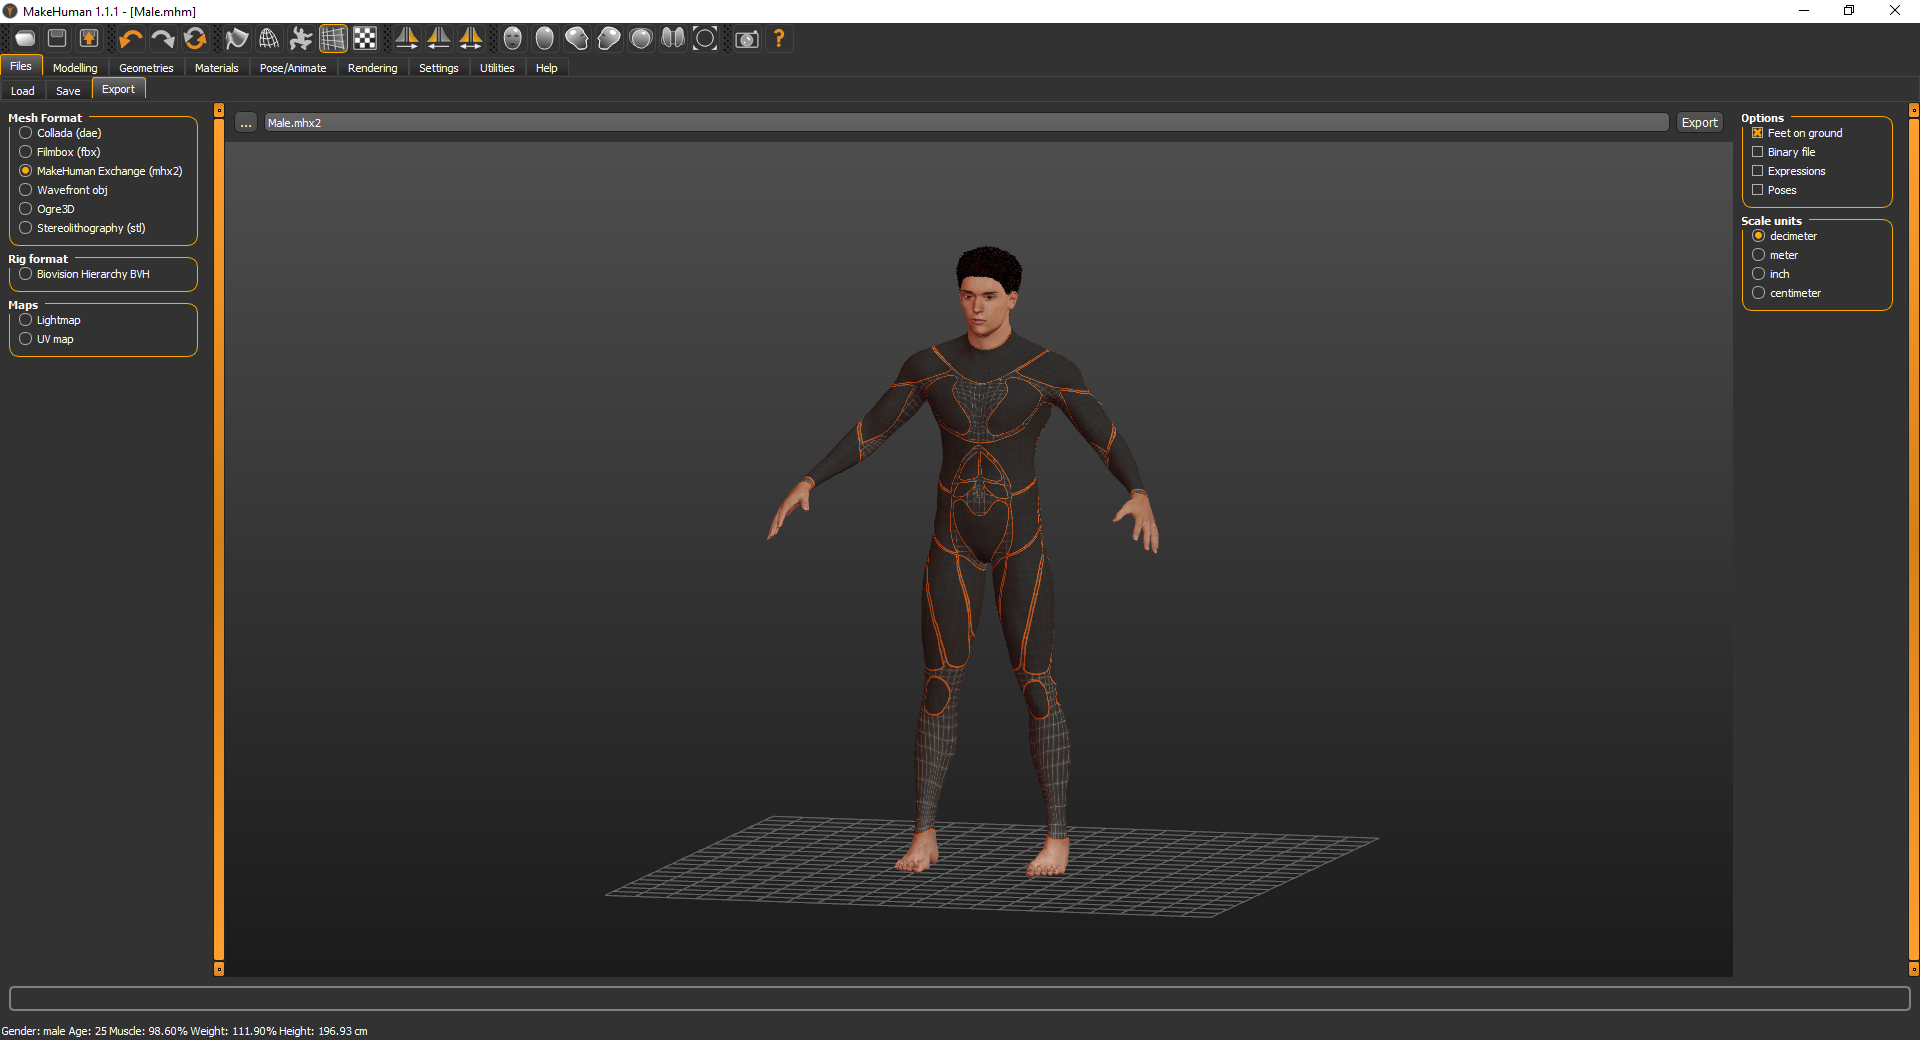
\includegraphics[width=0.6 \linewidth]{Male.png}
	\caption{Male.mhx2}
\end{figure}

\begin{figure}[h!]
	\centering
	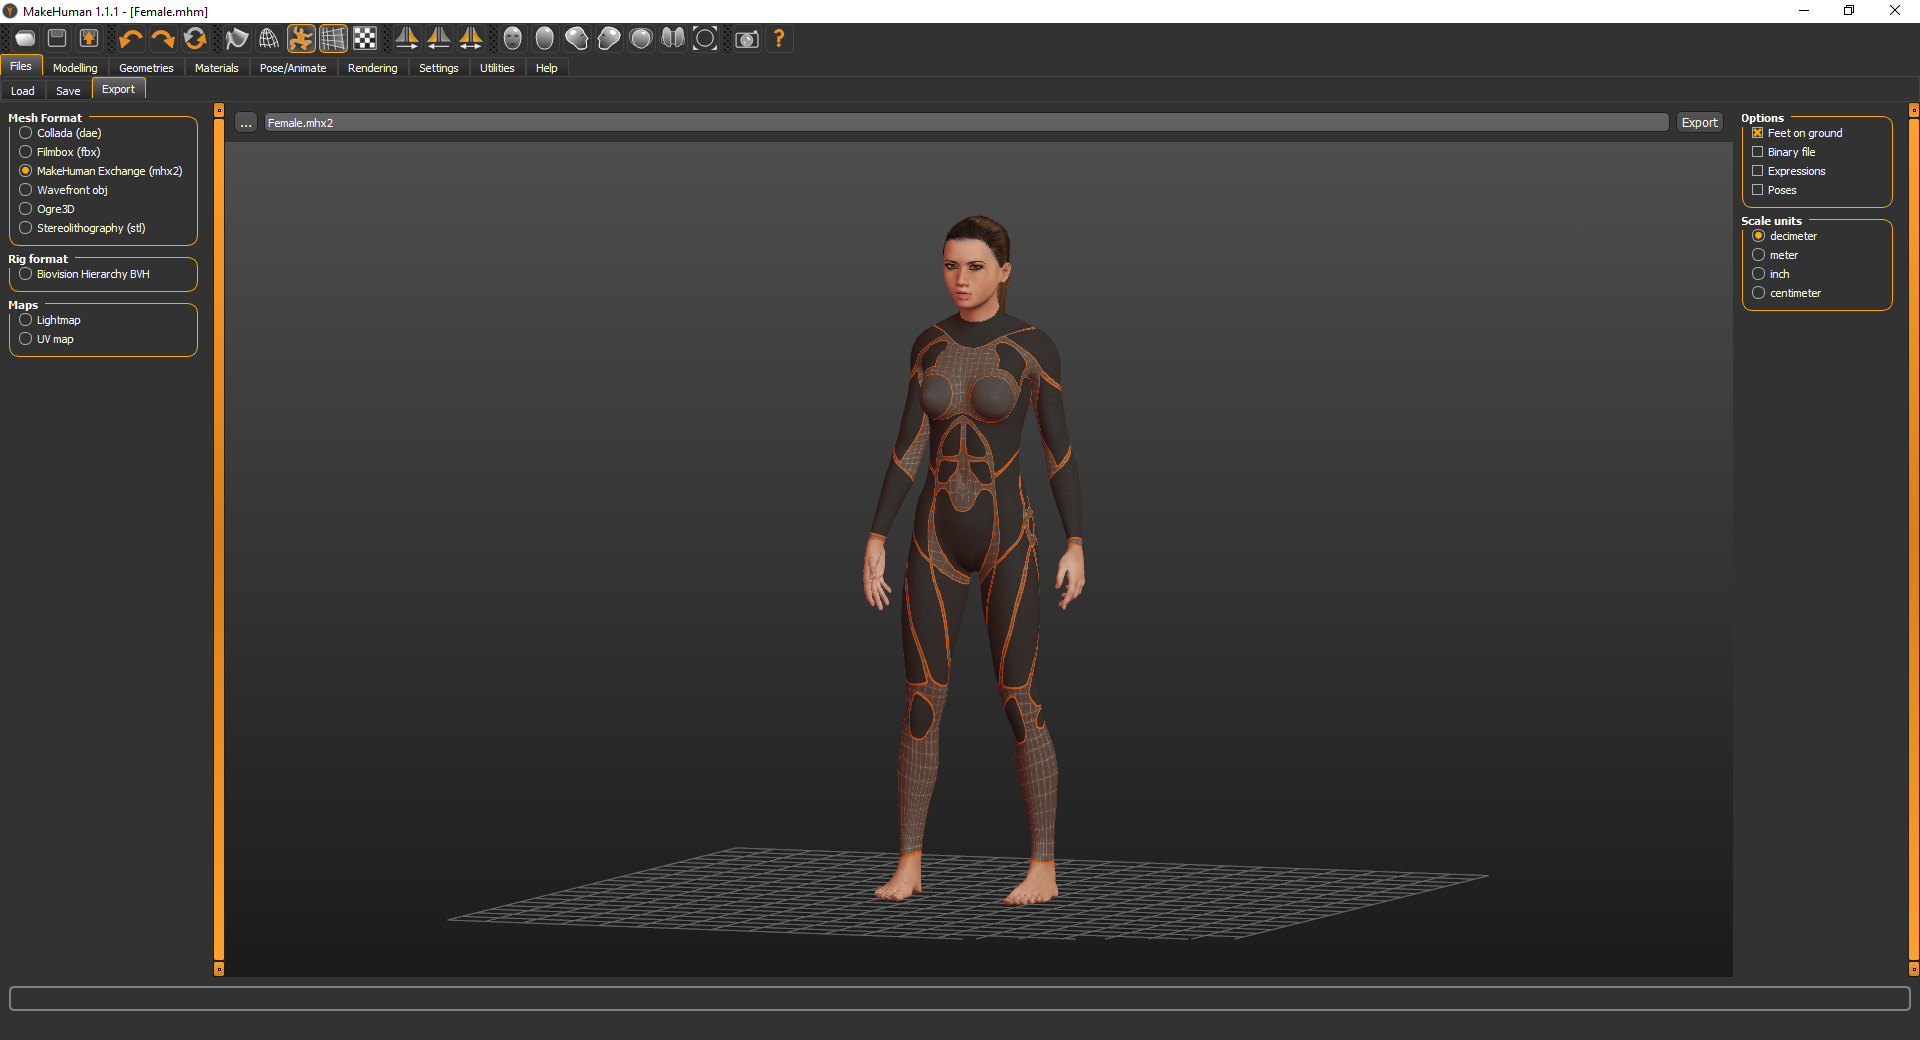
\includegraphics[width=0.6 \linewidth]{Female.png}
	\caption{Female.mhx2}
\end{figure}

\begin{figure}[h!]
	\centering
	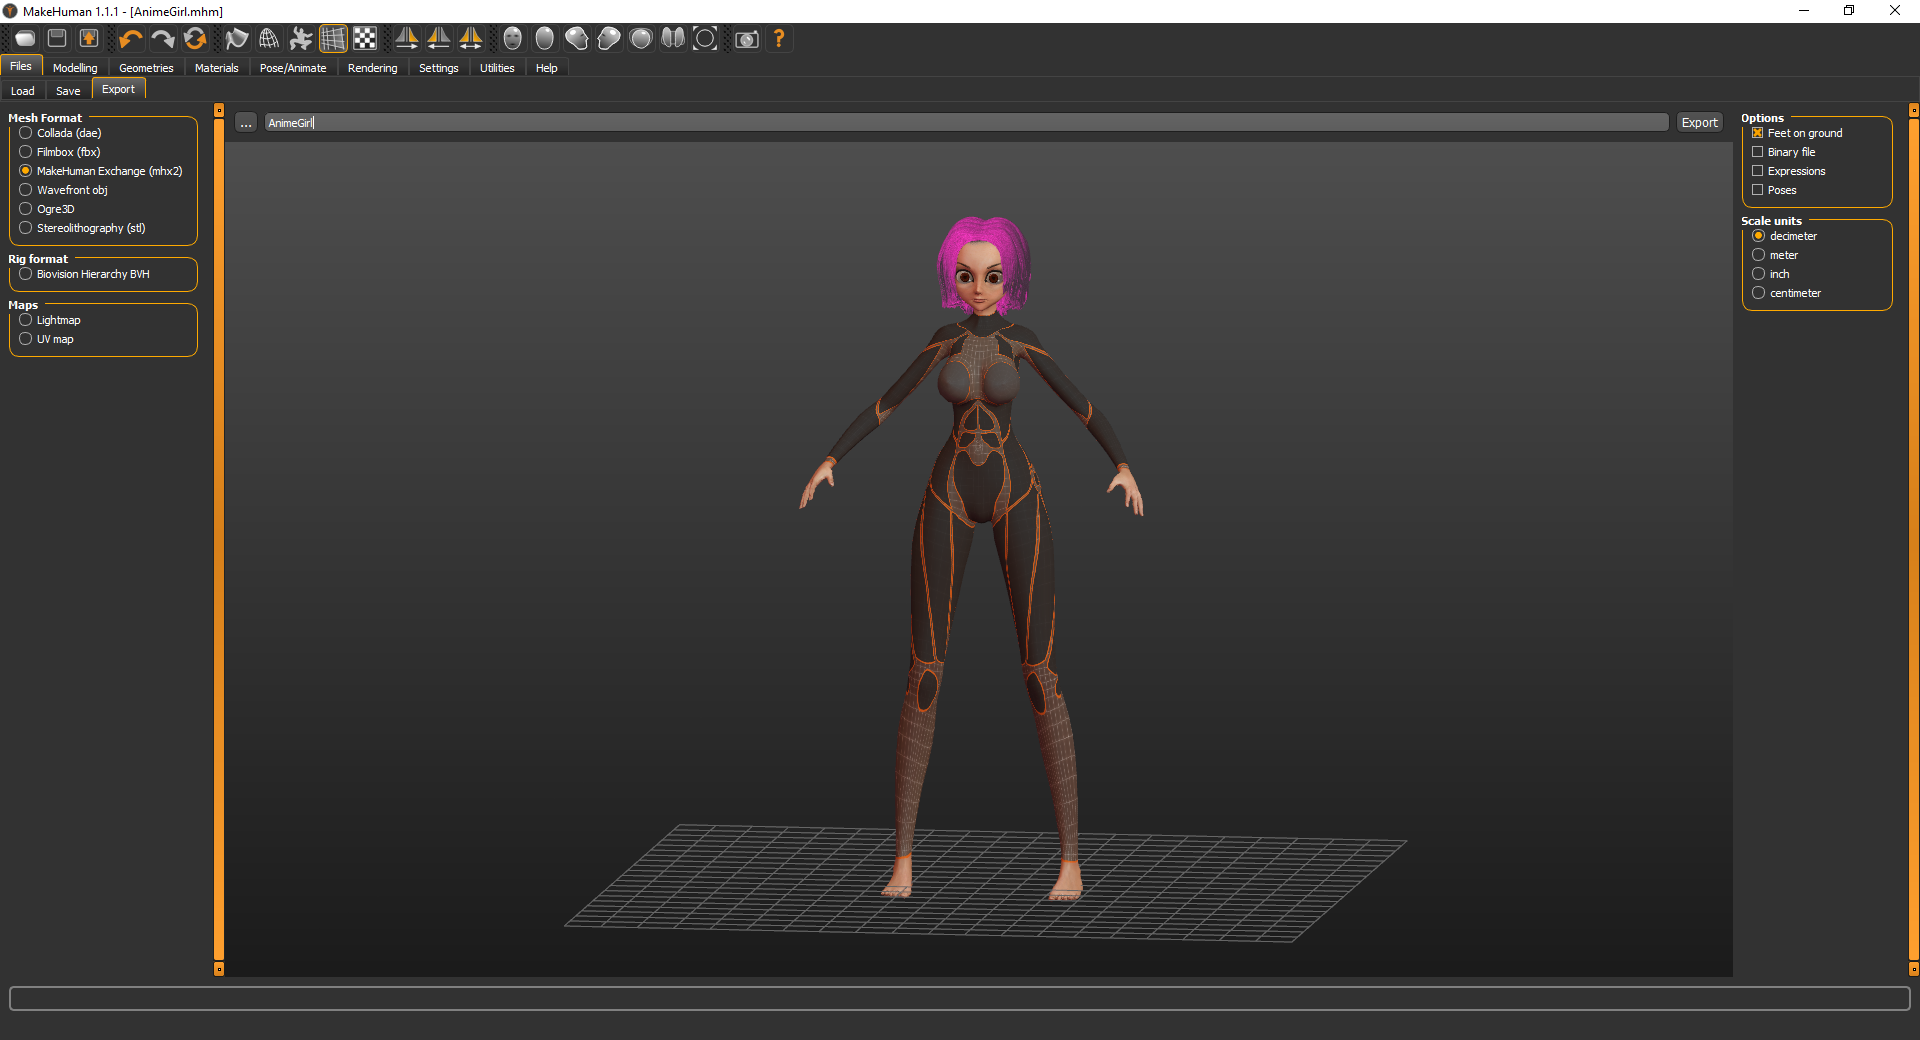
\includegraphics[width=0.6 \linewidth]{Anime.png}
	\caption{Anime.mhx2}
\end{figure}

\newpage
\subsection{Task 2.C}\label{sec:2C}


\begin{info} % Information block
	The models hair had to later be removed to successfully implement them.
\end{info}

\begin{figure}[h!]
	\centering
	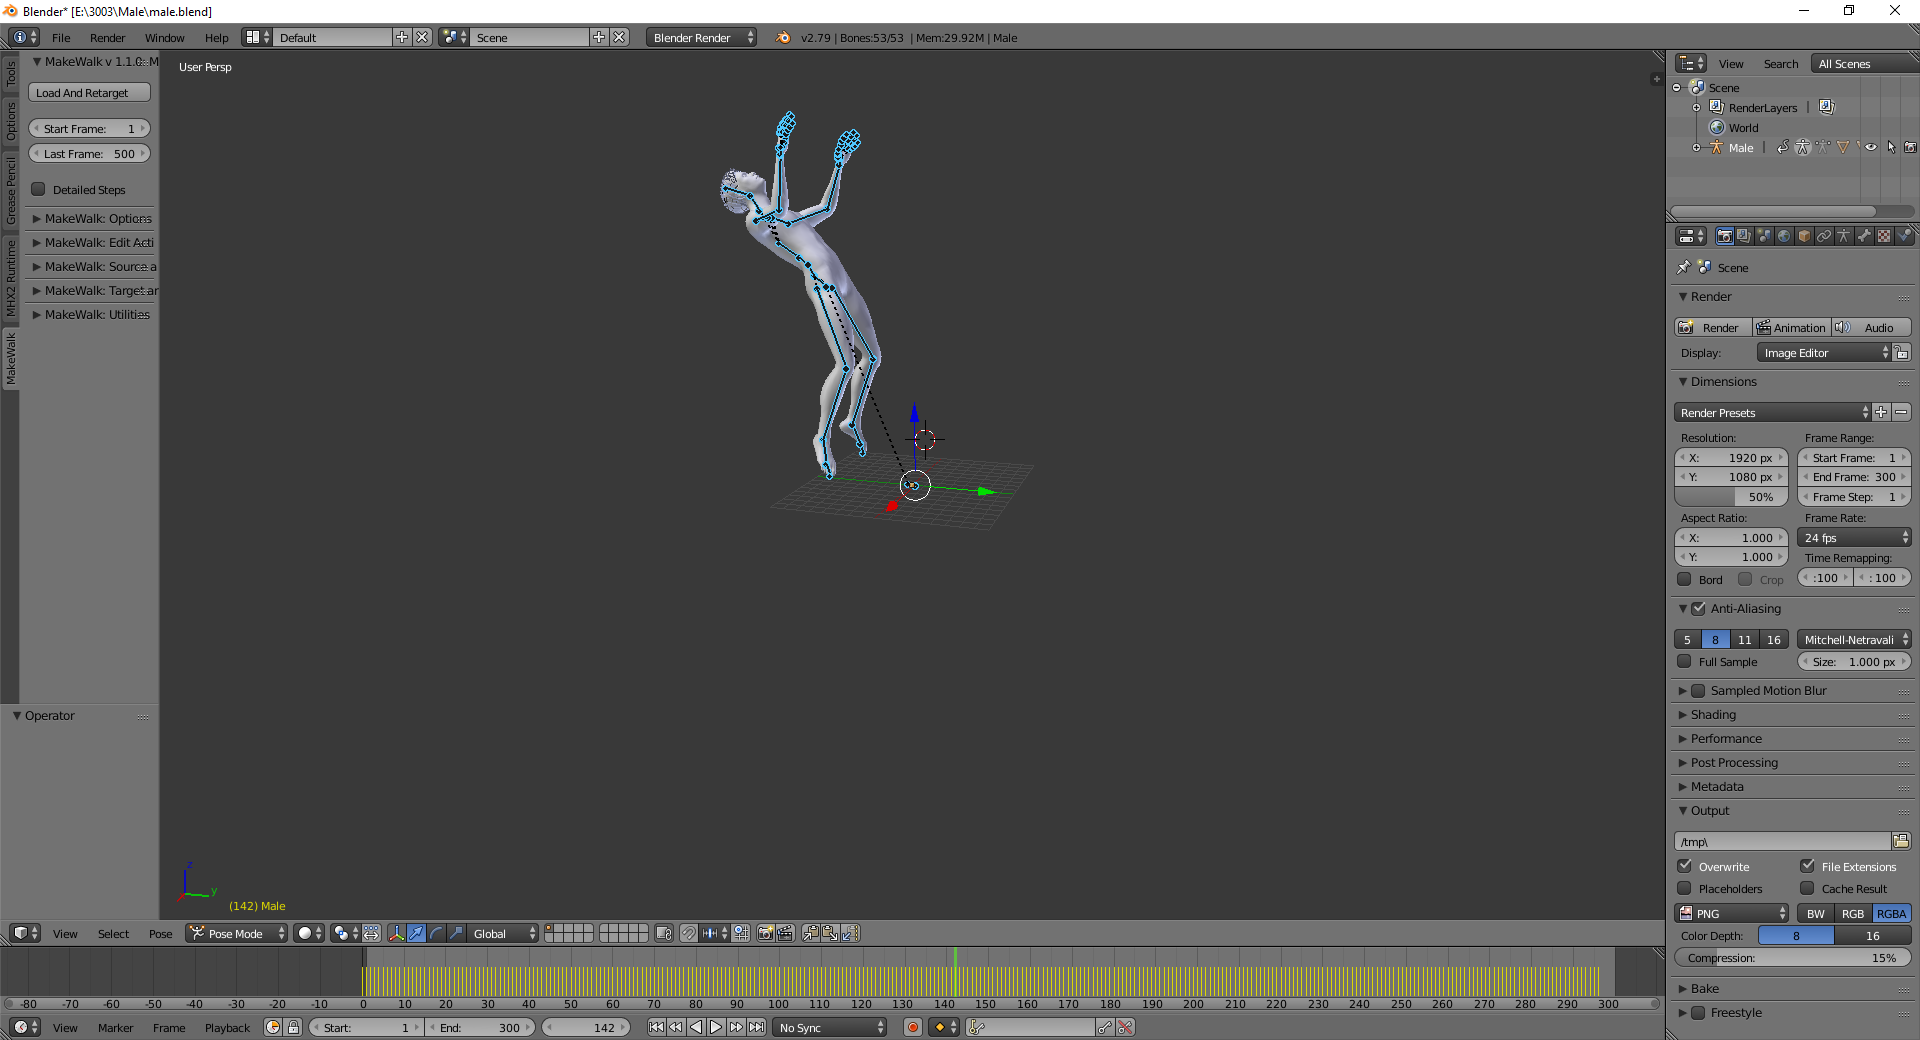
\includegraphics[width=0.6 \linewidth]{MaleAnimation.png}
	\caption{model57.x}
\end{figure}

\begin{figure}[h!]
	\centering
	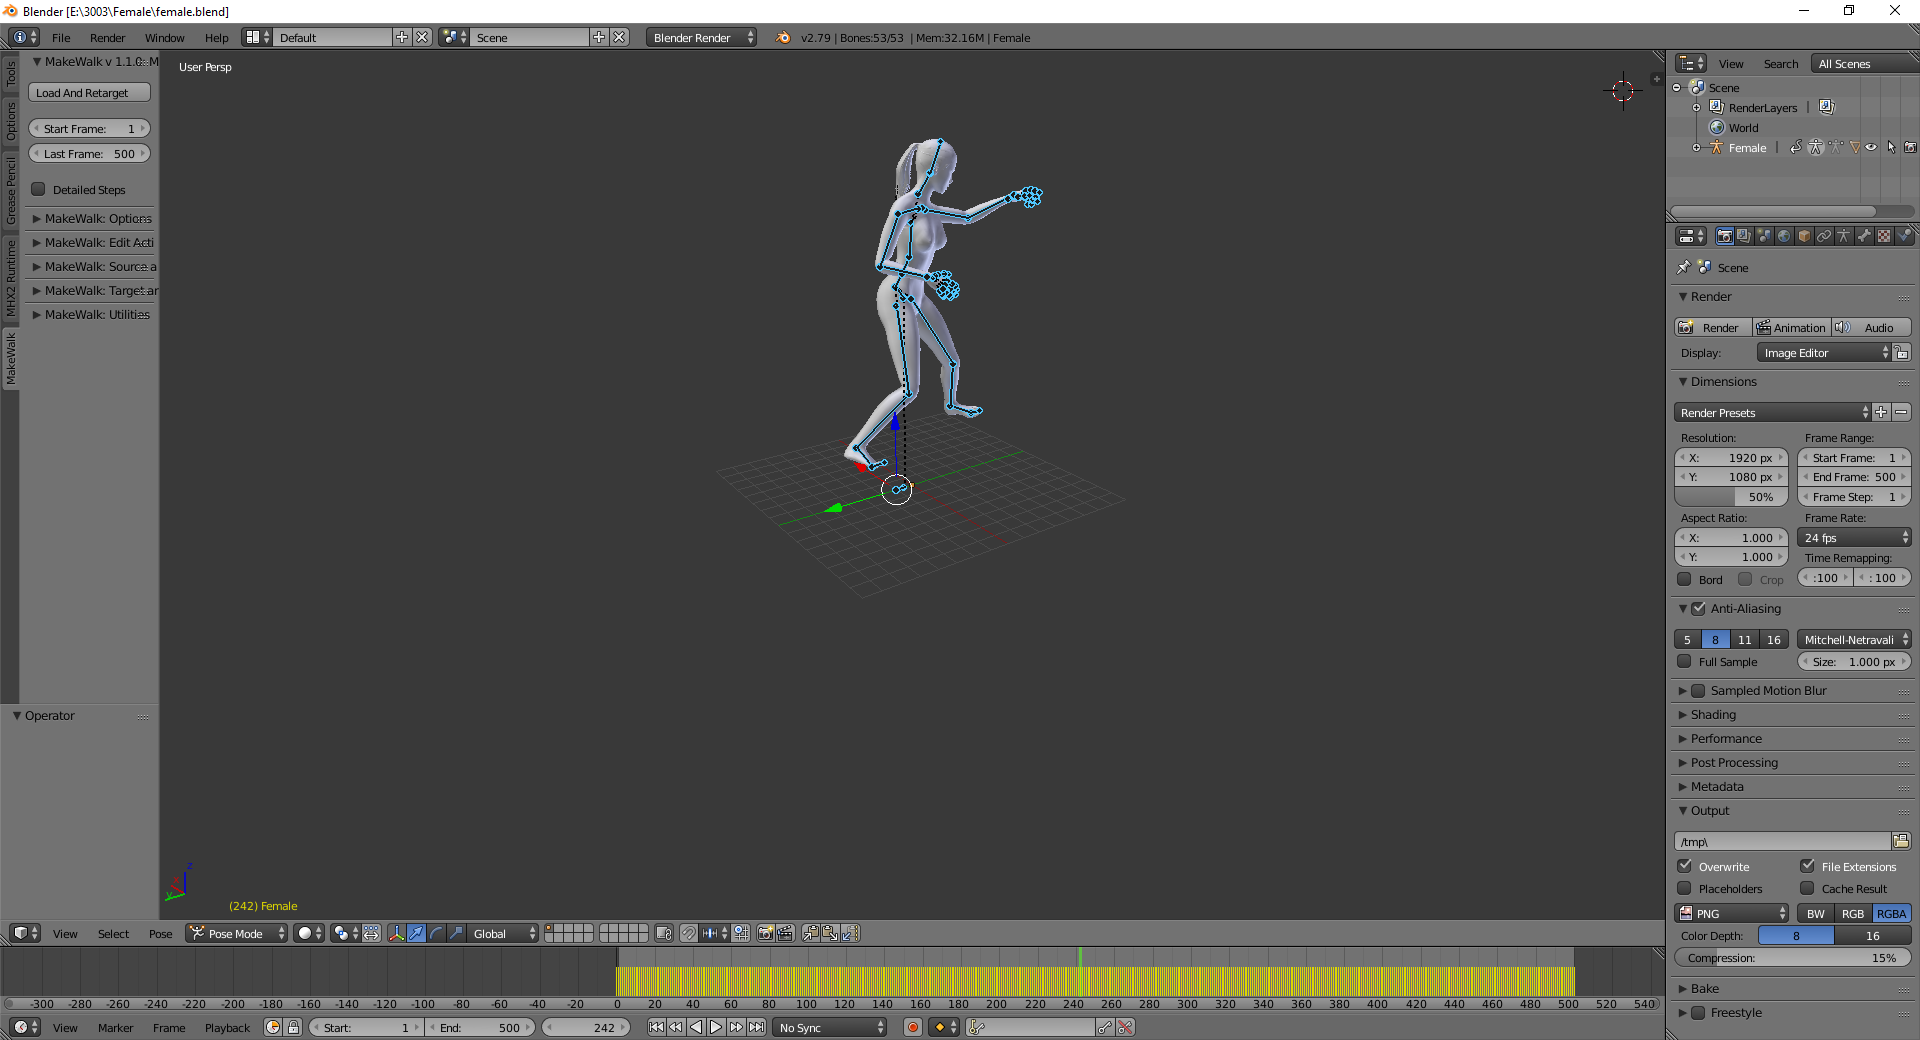
\includegraphics[width=0.6 \linewidth]{FemaleAnimation.png}
	\caption{model58.x}
\end{figure}

\begin{figure}[h!]
	\centering
	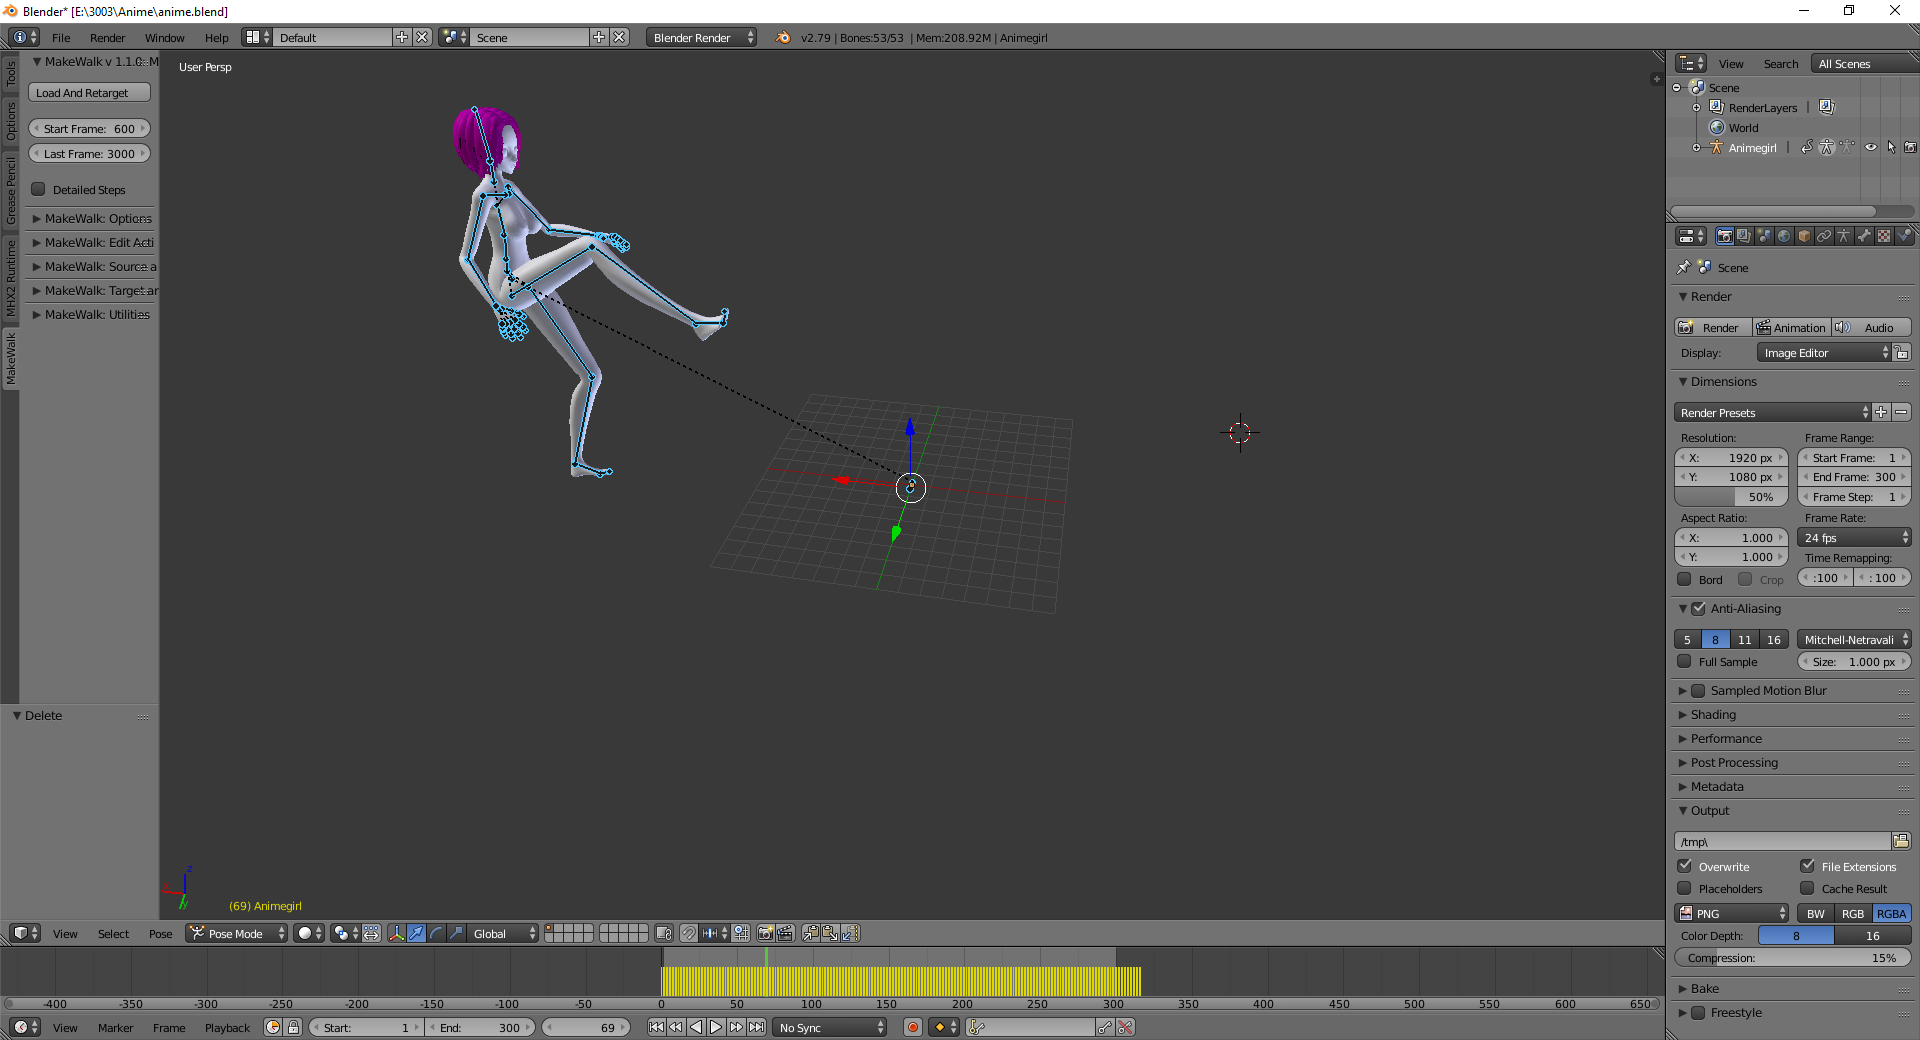
\includegraphics[width=0.6 \linewidth]{AnimeAnimation.png}
	\caption{model59.x}
\end{figure}

\newpage

\subsection{Task 2.D}\label{sec:2D}

\begin{figure}[h!]
	\centering
	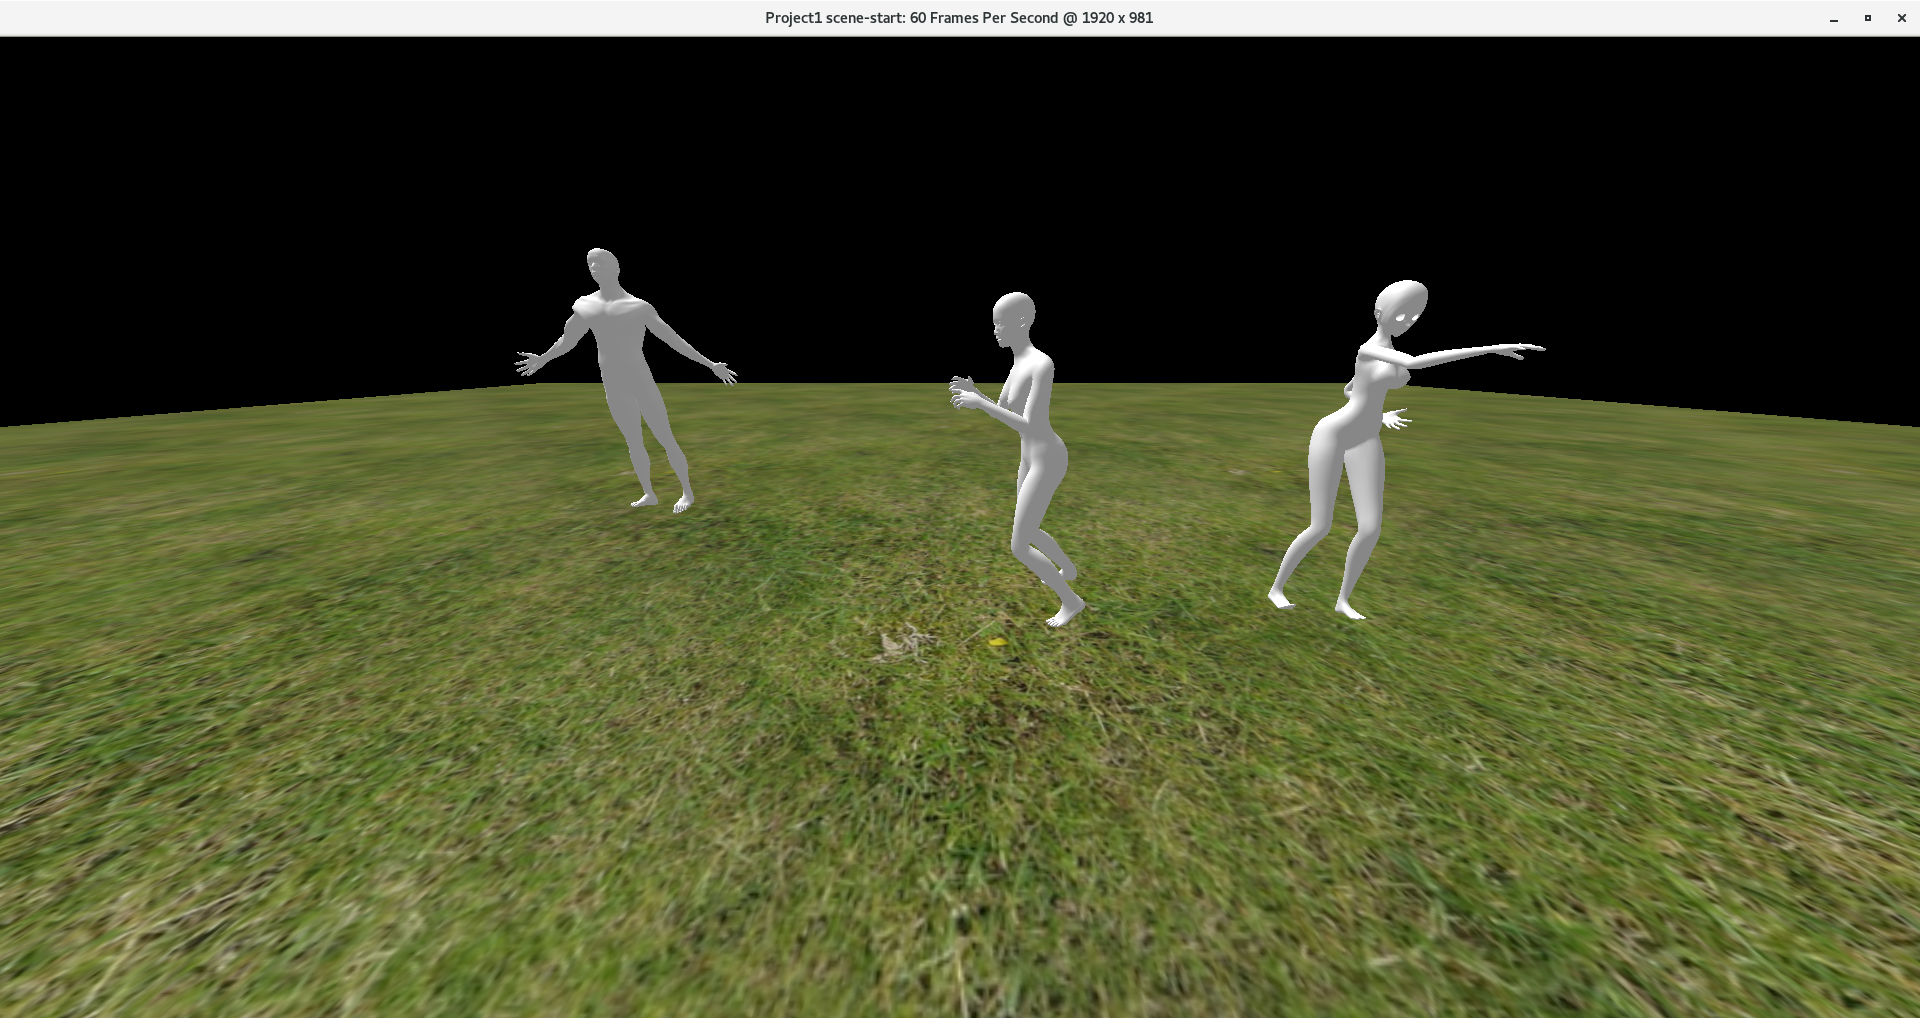
\includegraphics[width= \linewidth]{Animation.png}
	\caption{Animation Screenshot}
\end{figure}

\begin{commandlineG}
	\begin{verbatim}
	13. // Increased the number of meshes
	14. const int numMeshes = 60;
	\end{verbatim}
\end{commandlineG}

\begin{commandlineG}
	\begin{verbatim}
	109. // Added new mesh entries in the menu
	110. "57 (Added) Male", "58 (Added) Female", "59 (Added) Anime"};
	\end{verbatim}
\end{commandlineG}

\begin{commandline}
	\begin{verbatim}
	330. // Scaled the human models by a factor of 10x to have right size
	331. if (id > 0 && id < 55)
	332. {
	333.   sceneObjs[nObjects].scale = 0.005;
	334. }
	335. else if (id > 55)
	336. {
	337.   sceneObjs[nObjects].scale = 0.05;
	338. }
	\end{verbatim}
\end{commandline}

\begin{commandline}
	\begin{verbatim}
	352. // Rotated the models to face the right way when added to scene
	353. if (id > 55 && id < 59)
	354. {
	355.   // Human models turning right way
	356.   sceneObjs[nObjects].angles[0] = 0.0;
	357.   sceneObjs[nObjects].angles[1] = 0.0;
	358.   sceneObjs[nObjects].angles[2] = 0.0;
	359. }
	360. else if (id == 59)
	361. {
	362.   // Anime model turning right way
	363.   sceneObjs[nObjects].angles[0] = 0.0;
	364.   sceneObjs[nObjects].angles[1] = 90.0;
	365.   sceneObjs[nObjects].angles[2] = 0.0;
	366. }
	367. else
	368. {
	369.   // All other base models
	370.   sceneObjs[nObjects].angles[0] = 0.0;
	371.   sceneObjs[nObjects].angles[1] = 180.0;
	372.   sceneObjs[nObjects].angles[2] = 0.0;
	373. }
	\end{verbatim}
\end{commandline}


\begin{commandlineV}
	\begin{verbatim}
	28. // Animation of bones
	29. vec4 vpos = uBoneTransform * vec4(vPosition, 1.0);
	30. vec4 vnorm = uBoneTransform * vec4(vNormal, 0.0);
	\end{verbatim}
\end{commandlineV}

\begin{commandline}
	\begin{verbatim}
	82. // Added frames counter for animation of models
	83. int frames;
	\end{verbatim}
\end{commandline}

\begin{commandline}
	\begin{verbatim}
	95. // Declared variables for animation of model
	96. // Animation Speed begins at 4 to allow for adjustment within menu
	97. int frame = 0;
	98. int animationSpeed = 4;
	99. bool animationActive = true;
	\end{verbatim}
\end{commandline}



\begin{commandline}
	\begin{verbatim}
	381. // Added custom frame length for each animated human model
	382. if (id < 56)
	383. {
	384.   sceneObjs[nObjects].frames = 1;
	385. }
	386. else if (id == 56)
	387. {
	388.   sceneObjs[nObjects].frames = 300;
	389. }
	390. else if (id == 57)
	391. {
	392.   sceneObjs[nObjects].frames = 300;
	393. }
	394. else if (id == 58)
	395. {
	396.   sceneObjs[nObjects].frames = 500;
	397. }
	398. else if (id == 59)
	399. {
	400.   sceneObjs[nObjects].frames = 300;
	401. }
	\end{verbatim}
\end{commandline}


\begin{commandline}
	\begin{verbatim}
	534. // Adjusting animation speed through animationSpeed variable
	535. if (animationActive)
	536. {
	537.   // '10' used to allow tweaking of the animation speed
	538.   frame = glutGet(GLUT_ELAPSED_TIME) / (10 * animationSpeed) 
	% sceneObj.frames;
	539. }
	\end{verbatim}
\end{commandline}

\begin{commandline}
	\begin{verbatim}
	543. // Added frame variable to keep track of position time
	544. calculateAnimPose(meshes[sceneObj.meshId], scenes[sceneObj.meshId], 0,
	frame, boneTransforms);
	\end{verbatim}
\end{commandline}




\begin{commandline}
	\begin{verbatim}
	817. // Added new menu to allow for animation tweaking
	818. static void animationMenu(int id)
	819. {
	820.   // Pause and Play option
	821.   if (id == 100)
	822.   {
	823.     animationActive = !animationActive;
	824.   }
	825.   // Speed Down option
	826.   else if (id == 101)
	827.   {
	828.     animationSpeed += 1;
	829.   }
	830.   // Speed Up option
	831.   else if (id == 102)
	832.   {
	833.     // Limit the speed to above 1 so it cannot crash
	834.     if (animationSpeed > 1)
	835.     {
	836.       animationSpeed -= 1;
	837.     }
	838.   }
	839.   // Speed Reset option
	840.   else if (id == 103)
	841.   {  
	842.     animationSpeed = 4;
	843.   }
	844. }
	\end{verbatim}
\end{commandline}

\begin{commandline}
	\begin{verbatim}
	869. // Added sub-menu entry for Animation
	870. int animationMenuId = glutCreateMenu(animationMenu);
	871. glutAddMenuEntry("Pause / Play", 100);
	872. glutAddMenuEntry("Speed Down", 101);
	873. glutAddMenuEntry("Speed Up", 102);
	874. glutAddMenuEntry("Speed Reset", 103);
	\end{verbatim}
\end{commandline}

\begin{commandline}
	\begin{verbatim}
	887. // Added Animation main menu entry
	888. glutAddSubMenu("Animation", animationMenuId);
	\end{verbatim}
\end{commandline}


%---------------------------------------------------------------------------------------










\end{document}
